\documentclass{beamer}
\usepackage{sourcecodepro}
\usepackage[english]{babel}
\usepackage[utf8]{inputenc}
\usepackage{times}
\usepackage{amsmath,amsthm, amssymb, latexsym}
\usepackage{multicol}
\boldmath

\usepackage[orientation=portrait,size=a1,scale=1.4]{beamerposter}
\usetheme{LLT-poster}
\usecolortheme{ComingClean}

\title{NODAL: an Open Distributed Autotuning Library}
\author[phrb@ime.usp.br]{Pedro Bruel and Alfredo Goldman}
\institute{University of São Paulo, Brazil}
\date{\today}
\footimage{
\includegraphics[height=5cm]{usp}}

\begin{document}
\begin{frame}
\begin{columns}[t]
    \begin{column}{.46\linewidth}
        \begin{block}{\Large Autotuning with Cloud Computing}
            \large
            We modified OpenTuner to use Google Compute Engine (GCE) virtual machines as
            measurement servers:
            \begin{figure}[htpb]
                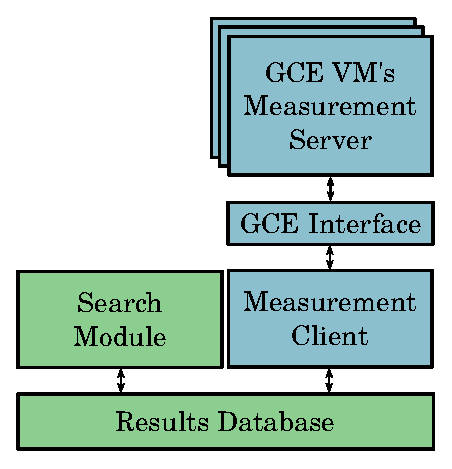
\includegraphics[width=0.45\linewidth]{high-level-implementation.eps}
                \caption{A}
            \end{figure}
        \end{block}
        \begin{block}{\Large Autotuning using Julia}
            \large
            \begin{figure}[htpb]
                
\includegraphics[width=0.84\linewidth]{logo}
            \end{figure}
            \begin{itemize}
                \item \textbf{Testbed:} GTX-980, GTX-750, Tesla-K40
                \item \textbf{Benchmark:} Rodinia, Vector Sum, Matrix Multiplication
                \item \textbf{Autotuning Tools:} OpenTuner Autotuning Framework
                \item \textbf{Fitness Value:} Mean of 30 executions
            \end{itemize}
        \end{block}
        \begin{block}{\Large Autotuning High-Level Synthesis for FPGAs with LegUp}
            \large
            \begin{itemize}
                \item \textbf{Testbed:} GTX-980, GTX-750, Tesla-K40
                \item \textbf{Benchmark:} Rodinia, Vector Sum, Matrix Multiplication
                \item \textbf{Autotuning Tools:} OpenTuner Autotuning Framework
                \item \textbf{Fitness Value:} Mean of 30 executions
            \end{itemize}
        \end{block}
    \end{column}
    \begin{column}{.46\linewidth}
        \begin{block}{\Large Results for the Rodinia Benchmark}
            \begin{itemize}
                \item \large{Almost \textbf{2.5x} speedup in one case}
            \end{itemize}
            \begin{figure}[htpb]
                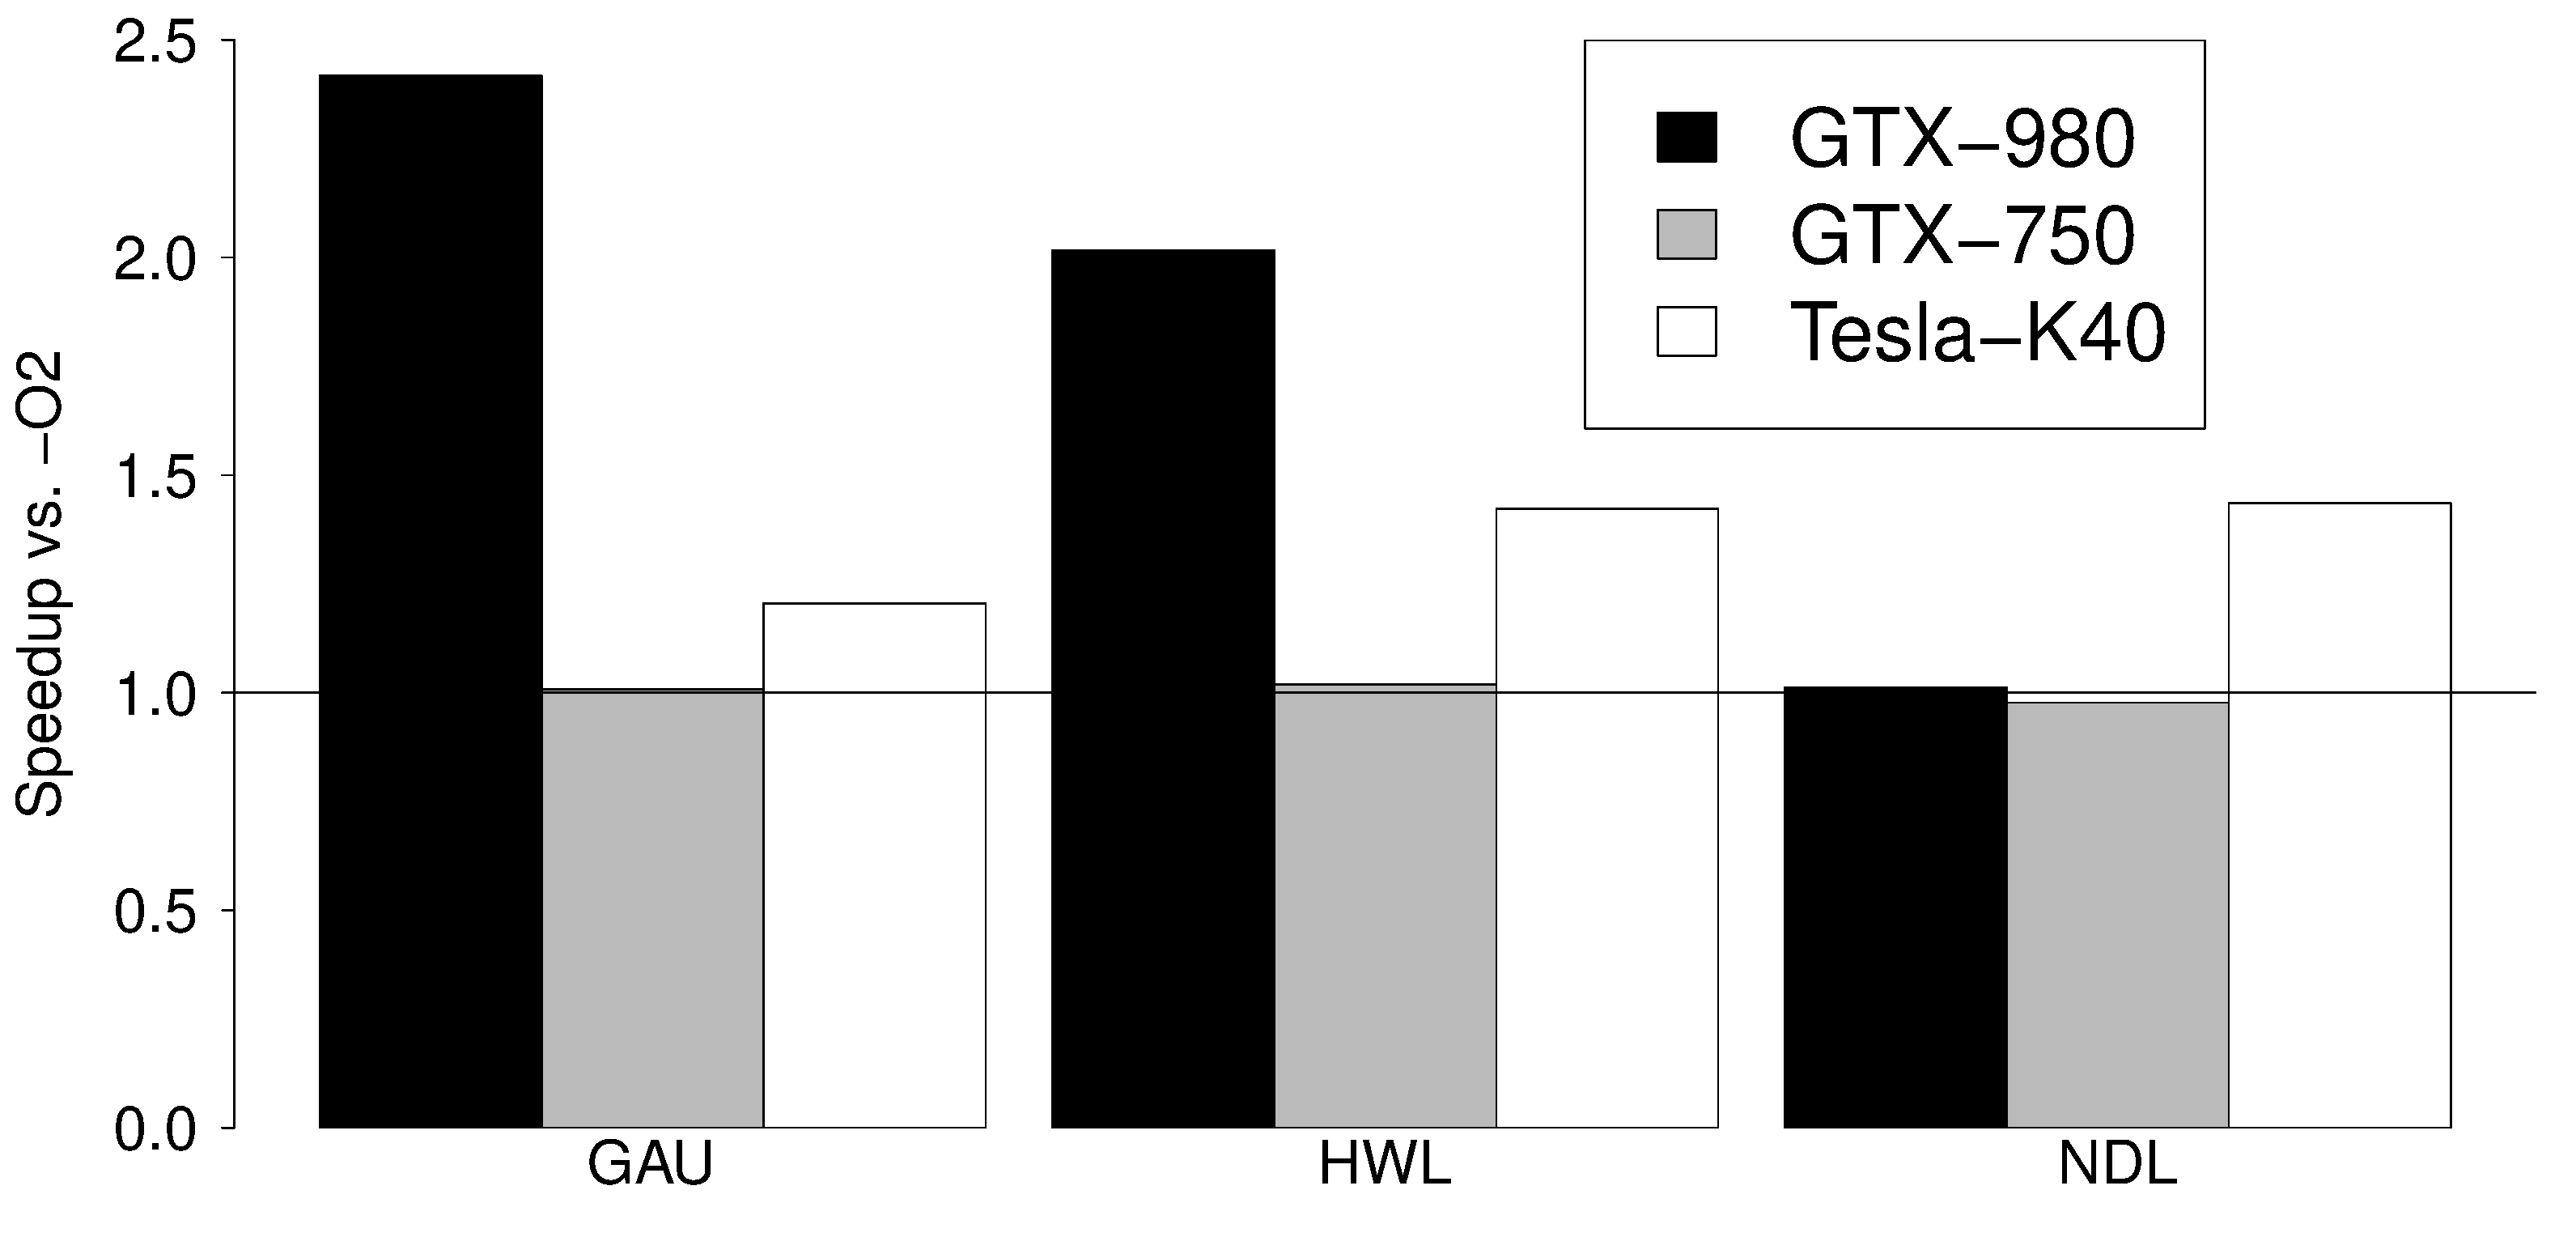
\includegraphics[width=0.84\linewidth]{RodiniaSummary.eps}
                \caption{A}
            \end{figure}
            \begin{itemize}
                \item \large{\textbf{Small} speedups in most cases}
            \end{itemize}
            \begin{figure}[htpb]
                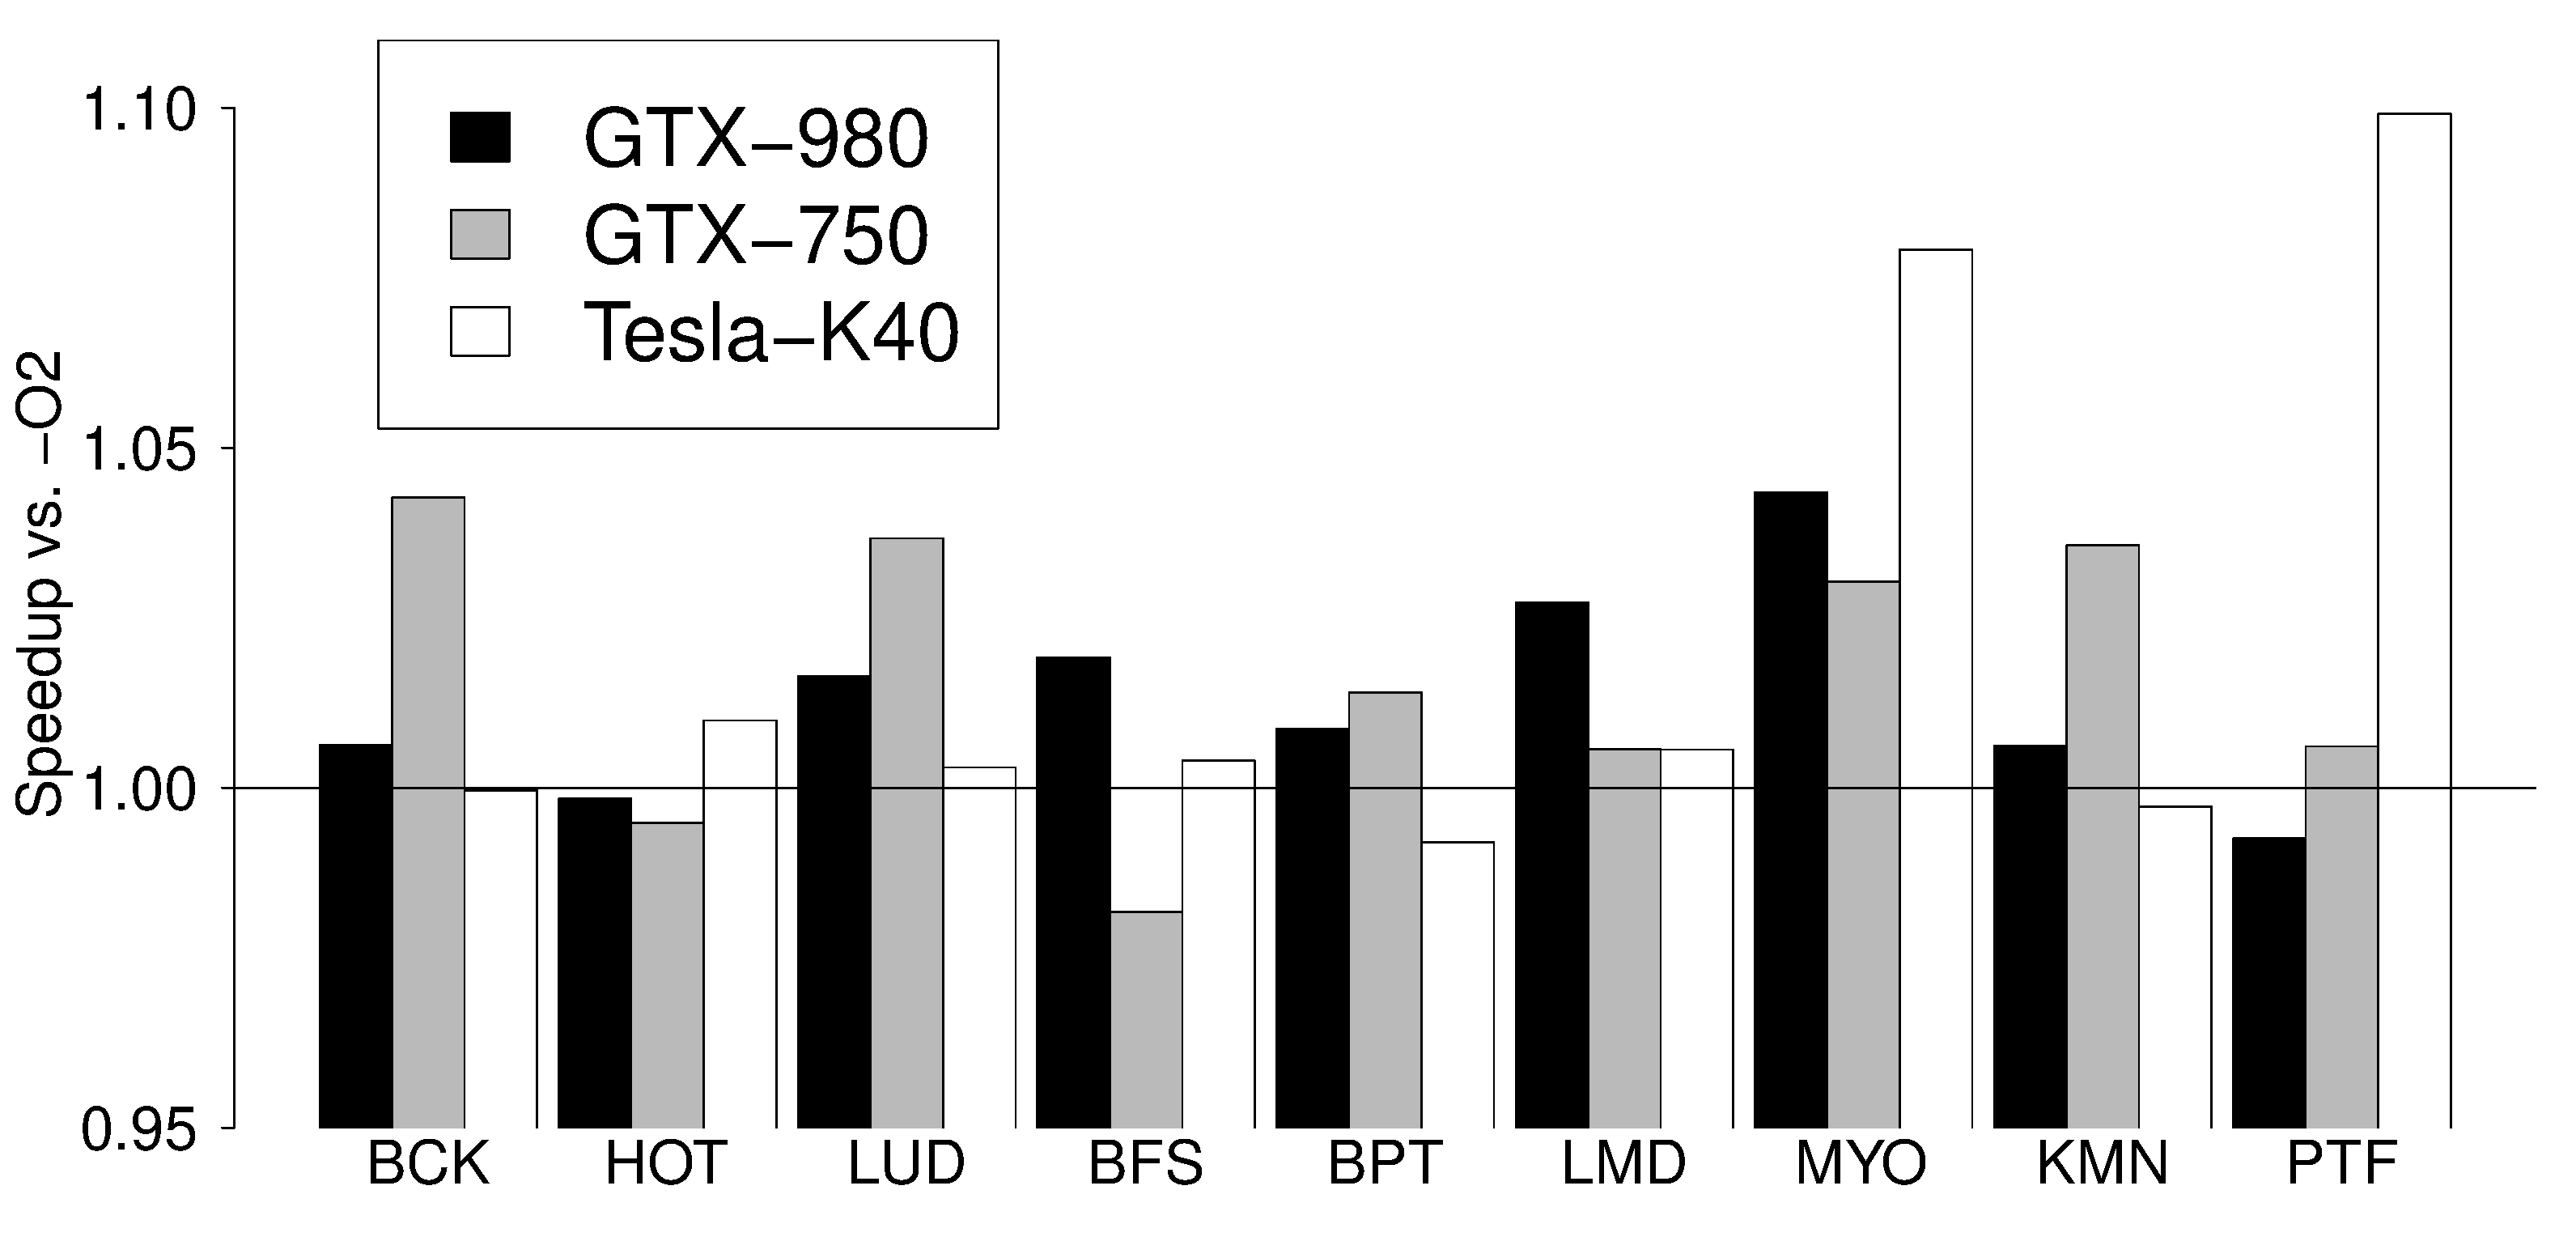
\includegraphics[width=0.84\linewidth]{RodiniaSummary_small.eps}
                \caption{A}
            \end{figure}
        \end{block}
        \begin{block}{\Large Conclusion}
            \large
            \begin{itemize}
                \item \textbf{Tuning Run:} 1h runs for each problem
                \item \textbf{Attempts to Cluster Results:} Not really successful
            \end{itemize}
        \end{block}
    \end{column}
\end{columns}
\end{frame}
\end{document}
